\documentclass[11pt,english]{beamer}

\usepackage[T1]{fontenc}
\usepackage[utf8]{inputenc}
\usepackage[main=french,english]{babel}
\usepackage{hyperref}
\usepackage{tikz}
\usetikzlibrary{shapes,snakes}
\usepackage{ulem}
\usepackage{xcolor, colortbl}
\usepackage{mathtools}
\usepackage{xcolor}

\usetikzlibrary{arrows}
\usetikzlibrary{positioning}


\usetheme{AnnArbor}
\usecolortheme{beaver}

\title{DeepVoice}                                          
\subtitle{Extracting meaningful signal representation for Speaker Recognition
  using deep architectures}

\author{Rémi Hutin, Rémy Sun, Raphaël Truffet \and Encadrants : Guillaume Gravier et Vedran Vukoki\'c}


\institute{ENS Rennes, IRISA}

\date{8 décembre 2016}


\AtBeginSection[]{
    \begin{frame}
        \frametitle{Sommaire}
        \tableofcontents[currentsection,hideothersubsections]
    \end{frame} 
}


\begin{document}

\begin{frame}
    \titlepage
\end{frame}

\begin{frame}
    \frametitle{Sommaire}
    \tableofcontents[hideallsubsections]
\end{frame}


\begin{frame}
  \frametitle{Signal processing workflow}
    \centering
    \begin{tikzpicture}[box/.style={draw,rounded corners,align=center}]
    \node[box,fill=blue!16] (a) {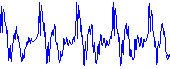
\includegraphics{signal.png}\\Signal};
    \end{tikzpicture}
\end{frame}

\begin{frame}
  \frametitle{Signal processing workflow}
    \centering
    \begin{tikzpicture}[box/.style={draw,rounded corners,align=center}]
    \node[box,fill=blue!16] (a) {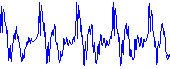
\includegraphics[scale=0.5]{signal.png}\\Signal};
    \node[box,fill=green!16,right =1cm of a] (f2) {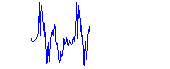
\includegraphics[scale=0.5]{fen2.png}};
    \node[box,fill=green!16,above =0.8cm of f2] (f1) {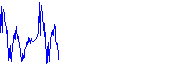
\includegraphics[scale=0.5]{fen1.png}};
    \node[below =0.8cm of f2] (f3) {\dots};
    \node[box,fill=green!16,below =0.8cm of f3] (fn) {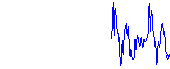
\includegraphics[scale=0.5]{fenn.png}};
    \draw[->] (a) -- (f1);
    \draw[->] (a) -- (f2);
    \draw[->] (a) -- (fn);
    \end{tikzpicture}
\end{frame}


\section{Signal representation for speaker recognition}

\begin{frame}
  \frametitle{Cesptral alanysis}
    \begin{figure}
    \centering
    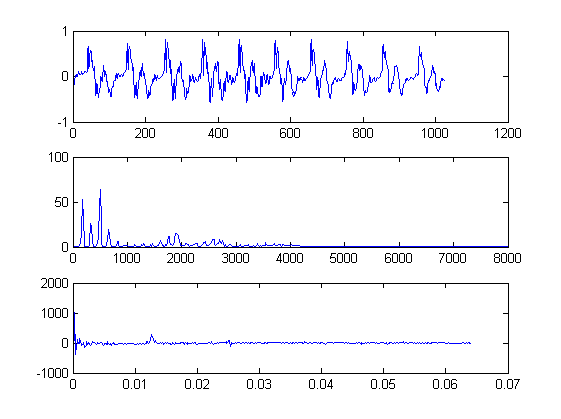
\includegraphics[trim={0 7.2cm 0 0}, clip, scale = 0.8]{cepstre.png}
    \end{figure}
      
    \begin{itemize}
    \item Hardly suitable for statistical modeling, distance calculation
    \item Apply a transformation :
    $ C(x(t)) = \mathcal{F}^{-1}(\ln(|\mathcal{F}(x(t))|)  $
    \item $C$ : cepstrum of the signal
    \item Cepstral domain : Euclidean distance
    \end{itemize}
  
\end{frame}



\begin{frame}
  \frametitle{Signal processing workflow}
    \centering
    \begin{tikzpicture}[box/.style={draw,rounded corners,align=center}]
    \node[box,fill=blue!16] (a) {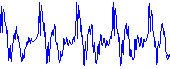
\includegraphics[scale=0.5]{signal.png}\\Signal};
    \node[box,fill=green!16,right =1cm of a] (f2) {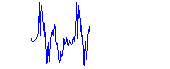
\includegraphics[scale=0.5]{fen2.png}};
    \node[box,fill=green!16,above =0.8cm of f2] (f1) {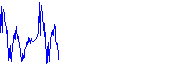
\includegraphics[scale=0.5]{fen1.png}};
    \node[below =0.8cm of f2] (f3) {\dots};
    \node[box,fill=green!16,below =0.8cm of f3] (fn) {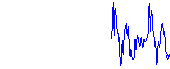
\includegraphics[scale=0.5]{fenn.png}};
    \draw[->] (a) -- (f1);
    \draw[->] (a) -- (f2);
    \draw[->] (a) -- (fn);
    
    
    
    \node[box,fill=orange!16, right = 1cm of f1] (c1) {cepstral coefficients};
    \node[box,fill=orange!16, right = 1cm of f2] (c2) {cepstral coefficients};
    \node[right = 3.5cm of f3] (c3) {\dots};
    \node[box,fill=orange!16, right = 1cm of fn] (cn) {cepstral coefficients};
    
    \draw[->] (f1) -- (c1);
    \draw[->] (f2) -- (c2);
    \draw[->] (fn) -- (cn);
    \end{tikzpicture}
\end{frame}

\begin{frame}
  \frametitle{Cepstral space}
  \begin{columns}
    \column{0.35\textwidth}
    \begin{itemize}
    \item Windowing
    \item Multiple cepstral representations
    \item High dimensional cepstral space tied to signal
    \item Probabilistic modeling
    \end{itemize}
    \column{0.6\textwidth}
    \only<1>{
      \begin{figure}
        \centering
        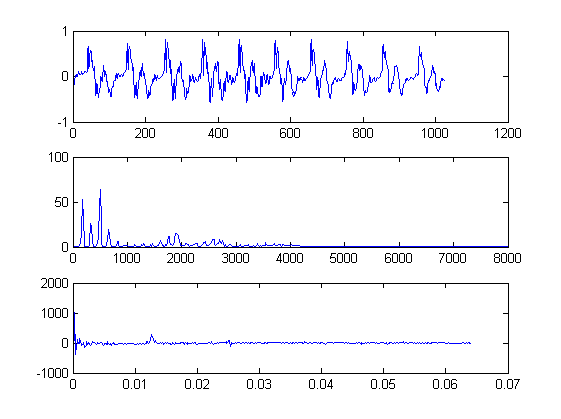
\includegraphics[scale = 0.5]{cepstre.png}
      \end{figure}
    }
    \only<2>{
      \begin{figure}
        \centering
       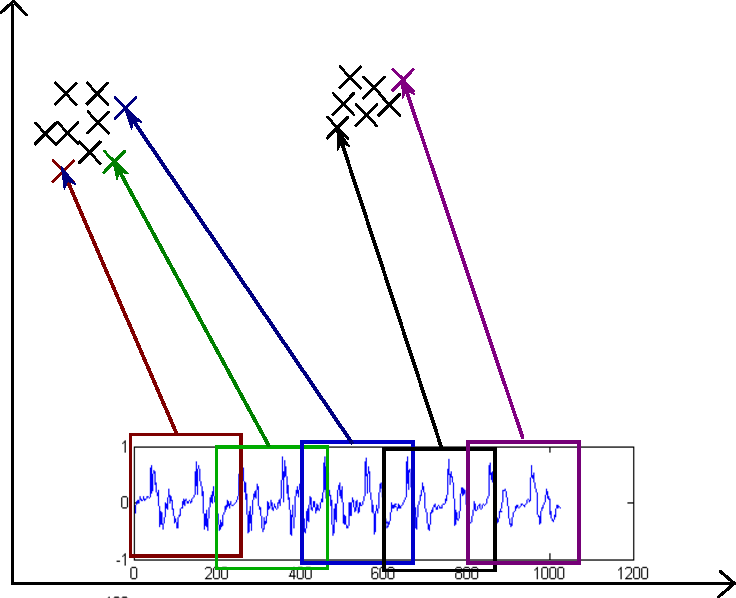
\includegraphics[scale = 0.5]{cepstral_space.pdf}
      \end{figure}
    }
  \end{columns}
\end{frame}

\begin{frame}
  \frametitle{Probabilistic modeling}
  \begin{columns}
    \column{0.35\textwidth}
    \begin{itemize}
    \item Model: gaussian combination
    \item Model: UBM standard
    \item<2> Adaptation to cepstral space
    \end{itemize}
    \column{0.6\textwidth}
    \only<1>{
      \begin{figure}
        \centering
       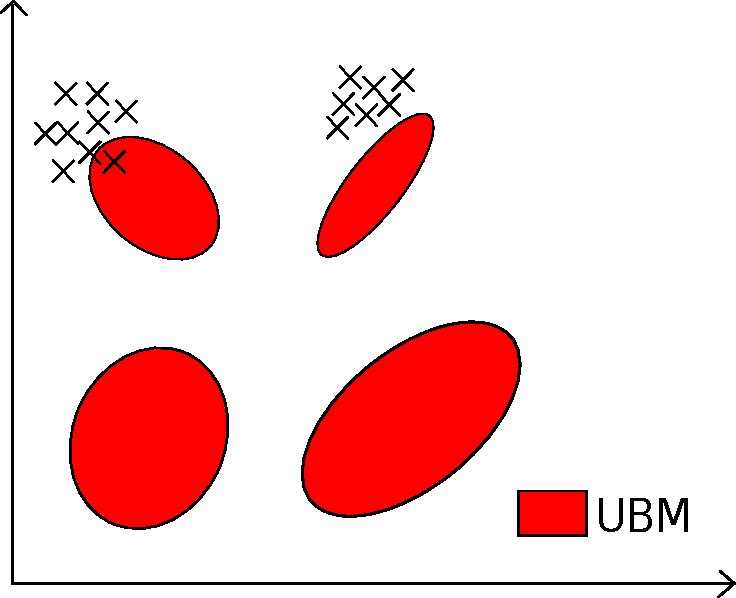
\includegraphics[scale = 0.5]{ubm.pdf}
      \end{figure}
    }
    \only<2>{
      \begin{figure}
        \centering
       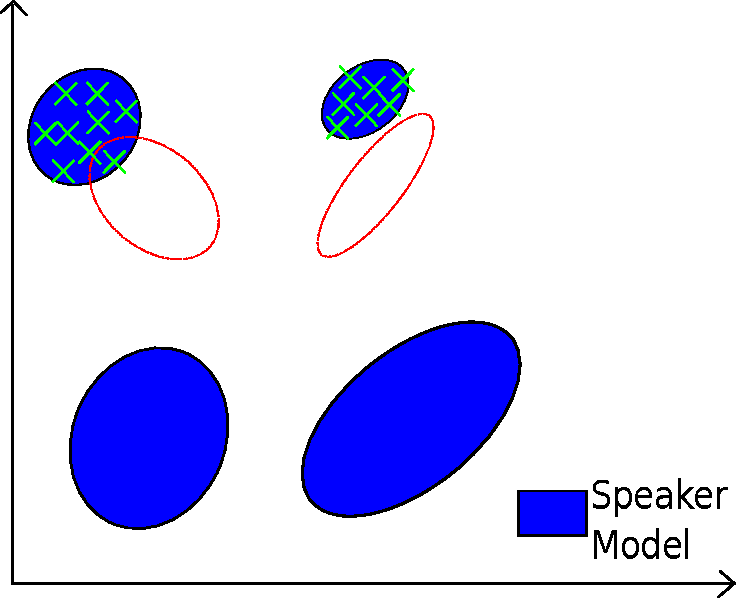
\includegraphics[scale = 0.5]{speker_model.pdf}
      \end{figure}
    }
  \end{columns}
\end{frame}

\begin{frame}
 \frametitle{supervectors}
  \begin{columns}
    \column{0.35\textwidth}
    \begin{itemize}
    \item Probabilistic model vector representation
    \item Represents the whole signal
    \item Spectral features
    \end{itemize}
    \column{0.6\textwidth}
    \begin{figure}
        \centering
       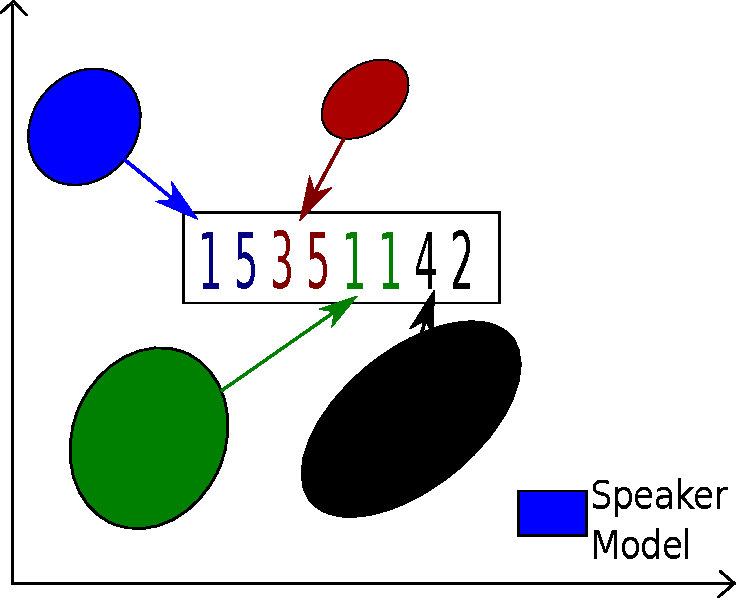
\includegraphics[scale = 0.5]{supervectors.pdf}
      \end{figure}
  \end{columns}
\end{frame}



\begin{frame}
  \frametitle{Signal processing workflow}
    \centering
    \begin{tikzpicture}[box/.style={draw,rounded corners,align=center}]
    
    \node[box,fill=green!16] (f2) {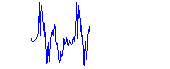
\includegraphics[scale=0.5]{fen2.png}};
    \node[box,fill=green!16,above =0.8cm of f2] (f1) {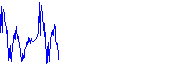
\includegraphics[scale=0.5]{fen1.png}};
    \node[below =0.8cm of f2] (f3) {\dots};
    \node[box,fill=green!16,below =0.8cm of f3] (fn) {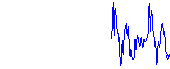
\includegraphics[scale=0.5]{fenn.png}};
    
    \node[box,fill=orange!16, right =1cm of f1] (c1) {cepstral coefficients};
    \node[box,fill=orange!16, right =1cm of f2] (c2) {cepstral coefficients};
    \node[below, right = 3.5cm of f3] (c3) {\dots};
    \node[box,fill=orange!16, right =1cm of fn] (cn) {cepstral coefficients};
    
    \draw[->] (f1) -- (c1);
    \draw[->] (f2) -- (c2);
    \draw[->] (fn) -- (cn);
    
    \node[box,fill=cyan!16, right = 2cm of c2] (sv) {Supervector};
    \node[box,fill=red!16, above = 1.5cm of sv] (ubm) {UBM};
    
    \draw[->] (c1) -- (sv);
    \draw[->] (c2) -- (sv);
    \draw[->] (cn) -- (sv);
    \draw[->] (ubm) -- (sv);
    \end{tikzpicture}
\end{frame}

\begin{frame}
  \frametitle{i-vectors}
  
\end{frame}

\begin{frame}
  \frametitle{i-vectors}
  
\end{frame}

\begin{frame}
  \frametitle{i-vectors}
  
\end{frame}

\begin{frame}
  \frametitle{Signal processing workflow}
    \centering
    \begin{tikzpicture}[box/.style={draw,rounded corners,align=center},barre/.style={draw,cross out,align=center}]
    
    \node[box,fill=orange!16] (c1) {cepstral coefficients};
    \node[box,fill=orange!16, below =0.8cm of c1] (c2) {cepstral coefficients};
    \node[below =0.8cm of c2] (c3) {\dots};
    \node[box,fill=orange!16, below =0.8cm of c3] (cn) {cepstral coefficients};
    
    
    \node[box,fill=cyan!16, right = 2cm of c2] (sv) {Supervector};
    \node[box,fill=red!16, above = 1.5cm of sv] (ubm) {UBM};
    
    \node[box,fill=yellow!16, right = 2cm of sv] (iv) {I-vectors};
    
    \draw[->] (c1) -- (sv);
    \draw[->] (c2) -- (sv);
    \draw[->] (cn) -- (sv);
    \draw[->] (ubm) -- (sv);
    
    \draw[->] (sv) -- (iv);
    
    \end{tikzpicture}
\end{frame}

\begin{frame}
  \frametitle{Signal processing workflow}
    \begin{tikzpicture}[box/.style={draw,rounded corners,align=center},barre/.style={draw,cross out,align=center}]
    
    \node[box,fill=orange!16] (c1) {cepstral coefficients};
    \node[box,fill=orange!16, below =0.8cm of c1] (c2) {cepstral coefficients};
    \node[below =0.8cm of c2] (c3) {\dots};
    \node[box,fill=orange!16, below =0.8cm of c3] (cn) {cepstral coefficients};
    
    
    \node[box,fill=cyan!16, right = 2cm of c2] (sv) {Supervector};
    \node[box,fill=red!16, above = 1.5cm of sv] (ubm) {UBM};
    
    \node[barre, right = 2cm of sv] (iv) {I-vectors};
    \node[box,fill=yellow!16, below = 1cm of iv] (ow) {\Large Our work};
    
    \draw[->] (c1) -- (sv);
    \draw[->] (c2) -- (sv);
    \draw[->] (cn) -- (sv);
    \draw[->] (ubm) -- (sv);
    
    
    
    \draw[->] (sv) -- (iv);
    \draw[->] (sv) -- (ow);
    
    \end{tikzpicture}
\end{frame}


\begin{frame}
  \frametitle{transition}
  
\end{frame}

\begin{frame}
  \frametitle{transition}
  
\end{frame}


\begin{frame}
  \frametitle{Signal processing workflow}
    \centering
    \begin{tikzpicture}[box/.style={draw,rounded corners,align=center},barre/.style={draw,cross out,align=center}]
    \node[box,fill=blue!16] (a) {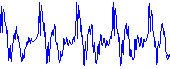
\includegraphics[scale=0.25]{signal.png}\\Signal};
    \node[box,fill=green!16,right =0.6cm of a] (f2) {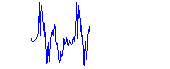
\includegraphics[scale=0.25]{fen2.png}};
    \node[box,fill=green!16,above =0.6cm of f2] (f1) {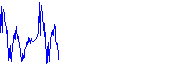
\includegraphics[scale=0.25]{fen1.png}};
    \node[below =0.8cm of f2] (f3) {\dots};
    \node[box,fill=green!16,below =0.6cm of f3] (fn) {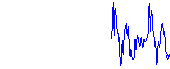
\includegraphics[scale=0.25]{fenn.png}};
    \draw[->] (a) -- (f1);
    \draw[->] (a) -- (f2);
    \draw[->] (a) -- (fn);
    
    
    
    \node[box,fill=orange!16, right = 0.6cm of f1] (c1) {cepstral\\coefficients};
    \node[box,fill=orange!16, right = 0.6cm of f2] (c2) {cepstral\\coefficients};
    \node[right = 2cm of f3] (c3) {\dots};
    \node[box,fill=orange!16, right = 0.6cm of fn] (cn) {cepstral\\coefficients};
    
    \draw[->] (f1) -- (c1);
    \draw[->] (f2) -- (c2);
    \draw[->] (fn) -- (cn);
    
    
    \node[box,fill=cyan!16, right = 0.6cm of c2] (sv) {Supervector};
    \node[box,fill=red!16, above = 1.5cm of sv] (ubm) {UBM};
    
    \draw[->] (c1) -- (sv);
    \draw[->] (c2) -- (sv);
    \draw[->] (cn) -- (sv);
    \draw[->] (ubm) -- (sv);
    
    \node[barre, right = 0.6cm of sv] (iv) {I-vectors};
    \node[box,fill=yellow!16, below = 1cm of iv] (ow) {\Large Our work};
    \draw[->] (sv) -- (iv);
    \draw[->] (sv) -- (ow);
    \end{tikzpicture}
\end{frame}
 

\section{Deep learning}

\begin{frame}
  \frametitle{Use of DNNs}
  
\end{frame}

\begin{frame}
  \frametitle{Formal neuron}
\def\layersep{2.5cm}


\begin{figure}
\centering
\begin{tikzpicture}[shorten >=1pt,->,draw=black!50, node distance=\layersep]
    \tikzstyle{every pin edge}=[<-,shorten <=1pt]
    \tikzstyle{neuron}=[ellipse,fill=black!25,minimum size=17pt,inner sep=0pt]
    \tikzstyle{input neuron}=[neuron, fill=green!50];
    \tikzstyle{output neuron}=[neuron, fill=red!50];
    \tikzstyle{hidden neuron}=[neuron, fill=blue!50];
    \tikzstyle{annot} = [text width=4em, text centered]

    % Draw the input layer nodes
    \foreach \name / \y in {1,...,4}
    % This is the same as writing \foreach \name / \y in {1/1,2/2,3/3,4/4}
        \node[input neuron, pin=left:] (I-\name) at (0,-\y) {$a_\y$};

    % Draw the hidden layer nodes
    \foreach \name / \y in {1,...,1}
        \path[yshift=-1.5cm]
            node[hidden neuron] (H-\name) at (\layersep,-\y cm) {};

    % Draw the output layer node
    \node[output neuron, right of=H-1] (O) {$e = f(WA + b)$};

    % Connect every node in the input layer with every node in the
    % hidden layer.
    \foreach \source in {1,...,4}
        \foreach \dest in {1,...,1}
            \path (I-\source) edge (H-\dest);

    % Connect every node in the hidden layer with the output layer
    \foreach \source in {1,...,1}
        \path (H-\source) edge (O);

    % Annotate the layers
    \node[annot,below of=H-1, node distance=1cm] (hl) {Weight $W$\\Bias $b$};
    \node[annot,above of=H-1, node distance=1cm] (hl) {Neuron};
    \node[annot,above of=I-1, node distance=1cm] (hl) {Input A};
\end{tikzpicture}

\end{figure}

  
\end{frame}

\begin{frame}
  \frametitle{Neural network}
\def\layersep{1.8cm}


\begin{figure}
\centering
\begin{tikzpicture}[shorten >=1pt,->,draw=black!50, node distance=\layersep]
    \tikzstyle{every pin edge}=[<-,shorten <=1pt]
    \tikzstyle{neuron}=[circle,fill=black!25,minimum size=17pt,inner sep=0pt]
    \tikzstyle{input neuron}=[neuron, fill=green!50];
    \tikzstyle{output neuron}=[neuron, fill=red!50];
    \tikzstyle{hidden neuron}=[neuron, fill=blue!50];
    \tikzstyle{hidden neuron back}=[neuron, fill=orange!50];
    \tikzstyle{annot} = [text width=4em, text centered]

    % Draw the input layer nodes
    \foreach \name / \y in {1,...,4}
    % This is the same as writing \foreach \name / \y in {1/1,2/2,3/3,4/4}
        \node[input neuron, pin=left:] (I-\name) at (0,-\y) {$a_\y$};

    % Draw the hidden layer nodes
    \foreach \name / \y in {1,...,5}
        {
        \visible<-11>{\path[yshift=0.5cm]
            node[hidden neuron] (H1-\name) at (\layersep,-\y cm) {};}
        \visible<12->{\path[yshift=0.5cm]
            node[hidden neuron back] (H1-\name) at (\layersep,-\y cm) {};}
        }
            
    \foreach \name / \y in {1,...,4}
        {
        \visible<-10>{\path
            node[hidden neuron] (H2-\name) at (2*\layersep,-\y cm) {};}
        \visible<11->{\path
            node[hidden neuron back] (H2-\name) at (2*\layersep,-\y cm) {};}
        }
            
    \foreach \name / \y in {1,...,5}
        {
        \visible<-9>{\path[yshift=0.5cm]
            node[hidden neuron] (H3-\name) at (3*\layersep,-\y cm) {};}
        \visible<10->{\path[yshift=0.5cm]
            node[hidden neuron back] (H3-\name) at (3*\layersep,-\y cm) {};}
        }
    % Draw the output layer node
    \node[output neuron,pin={[pin edge={->}]right:Output}, right of=H3-3] (O) {};

    % Connect every node in the input layer with every node in the
    % hidden layer.
    
    \foreach \source in {1,...,4}
        \foreach \dest in {1,...,5}
            {\only<\dest>{\path (I-\source) edge (H1-\dest);}}
            
            
    \visible<6->{
    \foreach \source in {1,...,4}
        \foreach \dest in {1,...,5}
            \path (I-\source) edge (H1-\dest);
    }
    
            
    \visible<7->{
    \foreach \source in {1,...,5}
        \foreach \dest in {1,...,4}
            \path (H1-\source) edge (H2-\dest);
    }
            
    \visible<8->{
    \foreach \source in {1,...,4}
        \foreach \dest in {1,...,5}
            \path (H2-\source) edge (H3-\dest);
    }
            
    \visible<9->{
    \foreach \source in {1,...,5}
        \path (H3-\source) edge (O);
    }
        
        
    % Annotate the layers
    \node[annot,above of=H1-1, node distance=1cm] (hl1) {Hidden layer 1};
    \node[annot,right of=hl1] (hl2) {Hidden layer 2};
    \node[annot,right of=hl2] (hl3) {Hidden layer 3};
    \node[annot,right of=hl3] {Output layer};
    \node[annot,left of=hl1] {Input layer};
    
    \node[annot,below of=H1-5, node distance=1cm] (wb1) {$W\visible<12->{'}_1$, $b\visible<12->{'}_1$};
    \node[annot,right of=wb1] (wb2) {$W\visible<11->{'}_2$, $b\visible<11->{'}_2$};
    \node[annot,right of=wb2] (wb3) {$W\visible<10->{'}_3$, $b\visible<10->{'}_3$};
\end{tikzpicture}

\end{figure}
  
\end{frame}

\begin{frame}
  \frametitle{Autoencoder}
  
\end{frame}

\begin{frame}
  \frametitle{Autoencoder}
  
\end{frame}

\begin{frame}
  \frametitle{i-vector 2.0}
  
\end{frame}

\section{Methods}

\begin{frame}
  \frametitle{Supplanting i-vectors}
  
  \begin{columns}
  \column{0.44\textwidth}  
  
\only<1>{
\begin{equation*}
    \begin{bmatrix}
      G_0^{0,0} \\   G_0^{0,1} \\ ... \\ G_{0}^{0,255} \\ G_0^{1,0} \\ .. \\ G_{0}^{N,255}
    \end{bmatrix}
\begin{bmatrix}
      G_1^{0,0} \\   G_1^{0,1} \\ ... \\ G_{1}^{0,255} \\ G_1^{1,0} \\ .. \\ G_{1}^{N,255}
    \end{bmatrix}
...
\begin{bmatrix}
      G_M^{0,0} \\   G_M^{0,1} \\ ... \\ G_{M}^{0,255} \\ G_M^{1,0} \\ .. \\ G_{M}^{N,255}
    \end{bmatrix}
  \end{equation*}
M supervectors
}

\only<2>{
  \begin{equation*}
    \begin{bmatrix}
      G_0^{0,0} \\   G_0^{0,1} \\ ... \\ G_{0}^{0,255} \\ G_0^{1,0} \\ .. \\ G_{0}^{N,255}
    \end{bmatrix}
  \end{equation*}
  Supervector from signal spoken by \textbf{someone}
}
  \column{0.5\textwidth}  
  What is needed to extract i-vectors ?
  \begin{itemize}
  \item Supervectors
  \item Training data (Labels on supervectors)
  \end{itemize}
  We will use the \textbf{exact same data}
  \end{columns}

\end{frame}

\begin{frame}
  \frametitle{Filtering out non-speaker noise} 
  \begin{columns}
    \column{0.5\textwidth}
    \begin{itemize}
    \item Filter out non-speaker dependant features
      \only<2-3>{(\textcolor{red}{noise})}
    \item<2-3> Need to denoise the signal
    \item<3> Same speaker, different signals     
    \item<3> Same signal, different non-speaker dependant noise
    \end{itemize}
    \column{0.4\textwidth}
    \only<1>{
      \begin{equation*}
        M = m + Tw
      \end{equation*}
}
\only<2>{
  \begin{equation*}
    M = \textcolor{red}{m} + T\color{green}{w}
  \end{equation*}
    }
  \end{columns}
\end{frame}

\begin{frame}
  \frametitle{Processed data}

  \begin{columns}
    \column{0.6\textwidth}
    \begin{itemize}
\setlength\itemsep{2em}
    \item \textbf{Raw data:} 15311 numeric soud files from BFMTV with labeled speakers
    \item \textbf{Pre-processed data:} 3 678 470 pairs $(v_1,v_2)$ of supervectors
      spoken by the same person
    \item \textbf{Input:} Supervector $v_1$ of length 9216
    \item \textbf{Output:} Supervector $v_2$ of length 9216

    \end{itemize}

    \column{0.35\textwidth}
    \only<1>{}
    \only<2>{
      \begin{equation*}
        \begin{bmatrix}
          v_1^{0,0} \\   v_1^{0,1} \\ ... \\ v_1^{0,255} \\ v_1^{1,0} \\ .. \\ v_1^{N,255}
        \end{bmatrix}
        \begin{bmatrix}
          v_2^{0,0} \\   v_2^{0,1} \\ ... \\ v_2^{0,255} \\ v_2^{1,0} \\ .. \\ v_2^{N,255}
        \end{bmatrix}
      \end{equation*}
    }
    \only<3>{
      \begin{equation*}
        \color{green}{
        \begin{bmatrix}
          v_1^{0,0} \\   v_1^{0,1} \\ ... \\ v_1^{0,255} \\ v_1^{1,0} \\ .. \\ v_1^{N,255}
        \end{bmatrix}
      }
      \color{black}{
        \begin{bmatrix}
          v_2^{0,0} \\   v_2^{0,1} \\ ... \\ v_2^{0,255} \\ v_2^{1,0} \\ .. \\ v_2^{N,255}
        \end{bmatrix}
        }
      \end{equation*}
    }
    \only<4>{
      \begin{equation*}
        \begin{bmatrix}
          v_1^{0,0} \\   v_1^{0,1} \\ ... \\ v_1^{0,255} \\ v_1^{1,0} \\ .. \\ v_1^{N,255}
        \end{bmatrix}
        \color{red}{
          \begin{bmatrix}
            v_2^{0,0} \\ v_2^{0,1} \\ ... \\ v_2^{0,255} \\ v_2^{1,0} \\ .. \\
            v_2^{N,255}
          \end{bmatrix}
}
      \end{equation*}
    }
  \end{columns}
  
\end{frame}

\begin{frame}
  \frametitle{Intermediate vector evaluation}
  \begin{columns}
    \column{0.6\textwidth}
    What uses i-vectors for speaker recognition?
    \begin{itemize}
      \setlength\itemsep{1em}
    \item Cosine similarity comparisons
    \item SVM
    \item Deep Neural networks
    \end{itemize}

    
    \only<2>{
      \textbf{Preliminary evaluation} with cosine similarity
    }

    \column{0.35\textwidth}
    \only<2>{
      \begin{itemize}\setlength\itemsep{2em}
      \item[] Threshold \textcolor{blue}{t}
      \item[] $distance \leq \textcolor{blue}{t}$ \textcolor{green}{same speaker}
      \item[] $distance \leq \textcolor{blue}{t}$
        \textcolor{red}{different speakers}
      \end{itemize}

    }
  \end{columns}

\end{frame}

\section{Discussion}

\begin{frame}
  \frametitle{Goals \only<2>{and expected issues}}
  What does it mean to improve on i-vectors?
  \begin{itemize}
  \item Better compression
    \only<2>{
      \begin{itemize}
      \item Compression size
      \item Hyperparameters
      \item Compromise with results
      \end{itemize}
    }
  \item Better results on angular treshold
    \only<2>{
      \begin{itemize}
      \item Optimization method
      \item Compromise with compression
      \end{itemize}
    }
  \item State-of-of-the-art-results
    \only<2>{
      \begin{itemize}
      \item Different training sets
      \item More complicated evaluation methods
      \end{itemize}
    }
  \end{itemize}
\end{frame}

\end{document}



